
%%%
% Any line that begins with a percent symbol is a comment. To compile
% this document and view the output:
%
% Run Latex
% Run Bibtex
% Then run Latex twice.
%
% This should produce the output PDF file named main.pdf
%%%

% This defines the style to use for this document.
% Do not modify.
\documentclass[letterpaper]{article}

% The following are akin to "import" statements in Python or Java -
% these import useful commands into the document for you to use.  You
% don't have to modify any of these lines. The AAAI package formats
% this document in the style of submissions to the American
% Association for Artificial Intelligence conference, one of the top
% AI conferences in the world. You will find that many academic
% publications in AI use this format.
\usepackage{aaai} 
\usepackage{times} 
\usepackage{helvet} 
\usepackage{courier} 
\setlength{\pdfpagewidth}{8.5in} 
\setlength{\pdfpageheight}{11in} 
\usepackage{amsmath}
\usepackage{amsthm}
\usepackage{graphicx}
\usepackage{graphics}
\usepackage{moreverb}
\usepackage{subfigure}
\usepackage{epsfig}
\usepackage{txfonts}
\usepackage{palatino}
\usepackage{algpseudocode}
\usepackage{multirow, multicol}
\usepackage{url}
\usepackage{tablefootnote}
\usepackage{color}

\setcounter{secnumdepth}{1}
\nocopyright

% Fill in your paper title, names and emails below
% The "\\" is used to break lines. The \url command
% is useful for typesetting URLs and email addresses (it uses the
% Courier font).
\title{Symbolic Regression with Genetic Programming}
 \author{Alden Hart \and Spencer Chadinha\\
 \url{{alhart, spchadinha}@davidson.edu}\\
 Davidson College\\
 Davidson, NC 28035\\
 U.S.A.}

% This is the "true" start of the document. All the text in your
% write-up should be placed within the \begin{document} and
% \end{document} decorators.
\begin{document}

\maketitle % formats the title nicely, do not modify

% While at this point you could just begin your write-up, often, it's
% useful to write each section of your write-up in a separate tex
% file (not unlike the modular decomposition you do for code you
% write). These \input commands insert the contents of the
% specified tex files in the order specified. Every write-up you
% submit must contain the following sections, in the shown order. Open
% each of the indicated tex files to understand what goes in each
% section, as well as for more TeX tips.
% Place the contents of your abstract between the
% \begin{abstract} and \end{abstract} decorators.

\begin{abstract}

Often described as "the second-best way to solve any problem", Genetic Programming (GP) relies on Darwinian principles of natural selection to produce models of a system. In this experiment, we applied GP to the problem of Symbolic Regression - that is, we attempted to find the function used to generate given datasets. To accomplish this, we randomly generated a population of symbol trees, each representing a different equation. We then evaluated the "fitness" of each tree and selected the fittest individuals to generate the next generation of trees. In doing so, we saw our algorithm produce a function that approximated data from Generator 1 with an absolute error of 5x$10^{-15}$. The resulting equation was 10/($x^2$ - 6x + 14), leading us to believe that this was, in fact, the equation used in Generator 1. Our algorithm was unable to accurately estimate a function for the dataset with three variables. Our best estimation for the function with three variables was: with an absolute error over 400 million.


This is noted later too, but as of the writing of this, our run of the three variable data hasn't finished running. From these results we have demonstrated that GP is a viable method of performing Symbolic Regression.\\

% The \textbf{} command makes the specified text bold. The \emph{} or
% \textit{} command are used to italicize text. In general, text is never
% underlined.

% DON'T FORGET TO MATCH EACH OPEN BRACE WITH A CLOSING BRACE!
\end{abstract}


% The \section{} command formats and sets the title of this
% section. We'll deal with labels later.
\section{Introduction}
\label{sec:intro}

Genetic programming, inspired by Darwinian evolution, uses the principles of natural selection, mutation, and reproduction, to explore a problem space. In this case, we use GP to perform Symbolic Regression and find the function used to generate a dataset. Symbolic Regression, a generalization of Linear Regression, is the process of finding an equation of best fit for an arbitrary dataset. While Linear Regression yields a linear formula, Symbolic Regression can be applied to find any function of any number of variables. The genetic programming approach is often thought of as a double-edged sword. On one hand, it can be adapted to solve almost any type of problem. On the other hand, it is a fairly uninformed solution method. It uses relatively little information about the problem to solve it, relying instead on guided randomness to deliver a suitable result. This randomness means the path taken to arrive at the solution is hidden to the user. GP may give a supremely accurate result, but yields no insight into why that result works, raising an important question: If you have the answer without knowing why it's right, have you really learned anything? \\
In the case of Symbolic Regression, how we arrive at a solution or why we chose certain steps is not as important as the function we produce. According to Koza, GP lends itself well to Symbolic Regression because it is error-driven learning \cite{Koza97geneticprogramming}.  It also finds unorthodox ways of discovering mathematical identities, which allows the use of a very limited set of operations to generate a wide range of functions.
In the following sections, we will discuss how we handled problems of diversity and overfitting, our results from SR with GP, and what we can conclude from our data.
. \\





\section{Background}
\label{sec:background}

\textbf{Initial Population}\\
	Diversity begins with the initial population. Both the size of the initial population and the method for generating an individual are extremely important to maintaining diversity. The size of the initial population must be large enough to be adequately dispersed across the problem space. Standard practice in the field of genetic programming is to have a population size of at least 500, although a larger population is always better \cite{poli08:fieldguide}We use a population of 500 in our experiments because of time constraints.\\

\textbf{Reproduction}\\
	Reproduction in symbolic regression passes an exact copy of a tree from one generation to the next. Failing to reproduce the most fit individual from one generation to the next could result in the loss of important functions from the population. We reproduce the top 10\% of our population for the next generation. This should keep the best genes in the previous population available for the current population, preventing loss of fitness between generations.\\

\textbf{Mutation}\\
	Mutation aids in maintaining diversity by introducing motifs into the population. Often, initial populations will not have all the parts necessary to arrive at an optimal solution, or a generation will lose a necessary part through random selection. Mutation offers a way for populations to recover lost or missing elements of optimal solutions. We used a point-mutation scheme, which could change operator nodes to different operations or alter the value of a terminal node. Point mutations help maintain diversity without introduce problems like overly complex tree structures which can lead to over-fitting of the data.\\

\textbf{Crossing over}\\
	Crossing over is the driving force behind improvement in genetic programming. Subtrees from two individuals that are deemed fit are combined together to generate a new individual. When crossing over two individuals, we randomly select subtrees from each individual and swap them between the two individuals.  We chose to randomly select crossover points in each individual to promote unique tree re-combinations. This is especially helpful for maintain diversity when two of the same individuals are crossed multiple times because the likelihood of generating the same child twice is extremely low.\\
	Selection of individuals for crossing over plays a large role in maintaining diversity. We implemented a very popular method known as tournament selection. This selection scheme randomly selects a subset of the current population and from that subset, picks the best individual to be a member of the next generation \cite{Gupta_anoverview}. We specifically chose this method of selection to prevent populations becoming composed of crossovers from a few fit individuals.\\

\textbf{Overfitting}\\
When implementing a machine learning algorithm such as GP, the experimenter must be wary of overfitting the training data. A model is said to overfit a dataset if it is specific only to those data. This results in a model that performs very well on the given set of training data, but does not generalize to data outside the training set. In the case of symbolic regression, any set of (x, y) pairs can be fit exactly by an arbitrarily complex polynomial. This does not mean, however, that you have found the actual function generating these points, and will give large errors when exposed to (x, y) pairs generated by that same function, but not included in the training set. To avoid this, we took several preventative measures. \\
Firstly, we implemented the most common technique to avoid overfitting, and split our data into a training set and a test set. We randomly selected 80\% of the total data to be our training set, leaving 20\% to be the test set. This way, when we ran ten iterations of GP, we had data that each best tree had not seen before. We determined the overall winner by evaluating each best tree on the test set.\\
Secondly, we implemented a dynamic depth-limiting strategy to prevent
overly complex hypotheses \cite{Overfitting}.  Since the underlying function was human-generated, we decided it was exceedingly unlikely that it be an extremely complex expression. Thus we limited the depth of trees in the population, weeding out overly complex hypotheses. This provided equations that were, on the whole, more generalizable and had similar test error and training error. In addition to limiting the depth, we also reduced the number of operators. This is discussed at length in the Experiment section, and greatly simplified trees.\\




\section{Experiments}
\label{sec:expts}

	To perform Symbolic Regression with GP on the
        data from Generator 1, we began with a population of 1,000
        randomly generated expression trees. An expression tree is a binary tree representing an expression that can be evaluated. The interior nodes of the tree can be any valid operation in the given language, and the leaf nodes can be any valid terminal, such as a constant or a variable name. Programming languages use expression trees to parse arithmetic and boolean expressions. In this case, the interior nodes of the
        trees were randomly selected from the set of valid operators,
        {+, *, /}. The leaf nodes of the trees were randomly selected
        from the set of valid terminals, consisting of the variable x
        and integer constants from -5 to 5. In order to reduce the
        number of constant trees (that is, trees that evaluated to a
        constant function), we decided that the variable x would be
        chosen with 50\% probability and a random choice from the set
        of integer constants would be chosen the remainder of the
        time. The problem at hand stated that the underlying function
        in Generator 1 used the operations +, -, *, /, and integer
        powers of x, but as a design consideration we chose to omit
        the operations – and exponentiation. We were able to do so
        because integer powers of x can be expressed through repeated
        multiplication, and subtraction is the addition of negative
        numbers, which are valid as terminals. Omitting these two
        operations greatly reduced the complexity of the trees
        produced by the algorithm, making it far more likely to
        produce an equation that would generalize well.\\

	To make a random tree, we began with a random operator node at
        the root and a predetermined depth limit of 10. We then built
        the rest of the tree recursively. Each node generated had a
        50\% chance of being a random terminal and ending that branch
        of the tree, or being a random operator. If the tree ever
        reached the depth limit, all new nodes were made to be
        terminals.\\

	Once the initial population was generated, we applied the
        GP algorithm. We allowed the algorithm to run
        for 35 generations, with the possibility of early termination
        if any tree's error was less than 0.2. To calculate error, we
        accumulated the absolute value of the difference between the
        tree'��s evaluation of a given x and the actual value, f(x). We
        chose this method over the squared error method because, like
        squared error, it never allows for negative error, but it also
        limits the possibility of the total error getting too large
        and causing an overflow.\\

	We used three different methods to generate a new
        generation. Firstly, the fittest 10\% of the population were
        duplicated into the next generation. This technique, called
        reproduction, ensures that every generation is at least as
        good as the preceding generation \cite{poli08:fieldguide}. Secondly, we
        mutated 10\% of the population. When a tree was selected for
        mutation, we traversed the tree, changing the current node
        40\% of the time. Terminals were only ever changed to other
        terminals, and operators to other operators. We determined the
        40\% node mutation rate through trial and error. Mutation
        occurred in place, so once a tree was mutated, it was still
        available to be picked for crossover. In another effort to
        keep diversity high, we used a tournament selection algorithm
        to select individuals for crossover. In tournament selection,
        we randomly select 10\% of the population and choose the
        fittest individual of those 10\% (the winner of the
        tournament). This probabilistically chose fitter individuals
        more frequently, but left open the possibility of a relatively
        unfit individual being chosen. When crossing over, we randomly
        selected a node in each tree and swapped the subtrees rooted
        at the nodes. To prevent overfitting, if the result of a
        crossover was too deep, we removed that individual and
        injected a new, random individual into the population. This
        limits the effects of overfitting by removing overly complex
        hypotheses and also contributed to diversity by adding random
        individuals periodically \cite{Gupta_anoverview}. We implemented a dynamic
        depth limit, where we defined "��too deep"�� as deeper than the
        fittest individual in the generation. We then continued
        crossing two trees until the new generation had the same
        number of individuals as the previous.\\

	When evaluating the trees, we split the initial dataset into a
        training set, containing roughly 80\% of the data, and a test
        set containing roughly 20\%. To divide the data, we generated
        a random number for each x value and assigned it and its
        corresponding f(x) value to either test or training depending
        on the value of the random number.\\

	After 35 generations, or when a tree's error dropped below
        0.2, we selected the fittest tree to be saved for comparison
        against the test set. We ran this process ten times to produce
        ten different winners. The final answer was the winner who
        performed best over the test data, giving us an estimate of
        the underlying equation behind the dataset.\\
        
        We then adapted our program to handle the function of three variables. We pared the original 100,000 point dataset down to a training and test set, each consisting of 50,000 randomly chosen points. We then performed the same algorithm, generating and evolving populations of trees for 35 generations or until a suitably accurate tree was found.




\section{Results}
\label{sec:results}

     To evaluate our data, we took a subset of the Generator 1 data
and split it into training and test sets. We noticed that the
data varied very little outside the range [-50, 50], so we
considered x-values from [-50,50] in increments of 0.1, and
their corresponding y-values.\\

Our algorithm produced spectacular results, finding an equation for
the Generator 1 data with less than 5 x 10-15 total error on the test
set. When evolving, this tree took 19 generations to be formed. After
19 generations, the equation  $$\frac{10}{x^2-6x+14}$$  had a total error of
less than 2x10-14 when evaluated on the test set, as stated above, the
error was similarly low. This indicates that the equation generalizes
well and was not overfit to the training data.\\

After ten runs of GP, we had ten trees that were each the best in that iteration of the algorithm. On average, one of these winning trees had an error of 31.27 on the test set with a standard deviation of 22.34. When considered in the scope of the size of the test set, these results are quite impressive. An error of 31 means that over the 200 datapoints in the test set, the derived function generated values that were on average 0.15 off from the actual values.\\

\begin{figure}[htb]

  \centering  % centers the image in the column

  % replace the second argument below with your filename. I like to
  % place all my figures in a sub-directory to keep things organized
  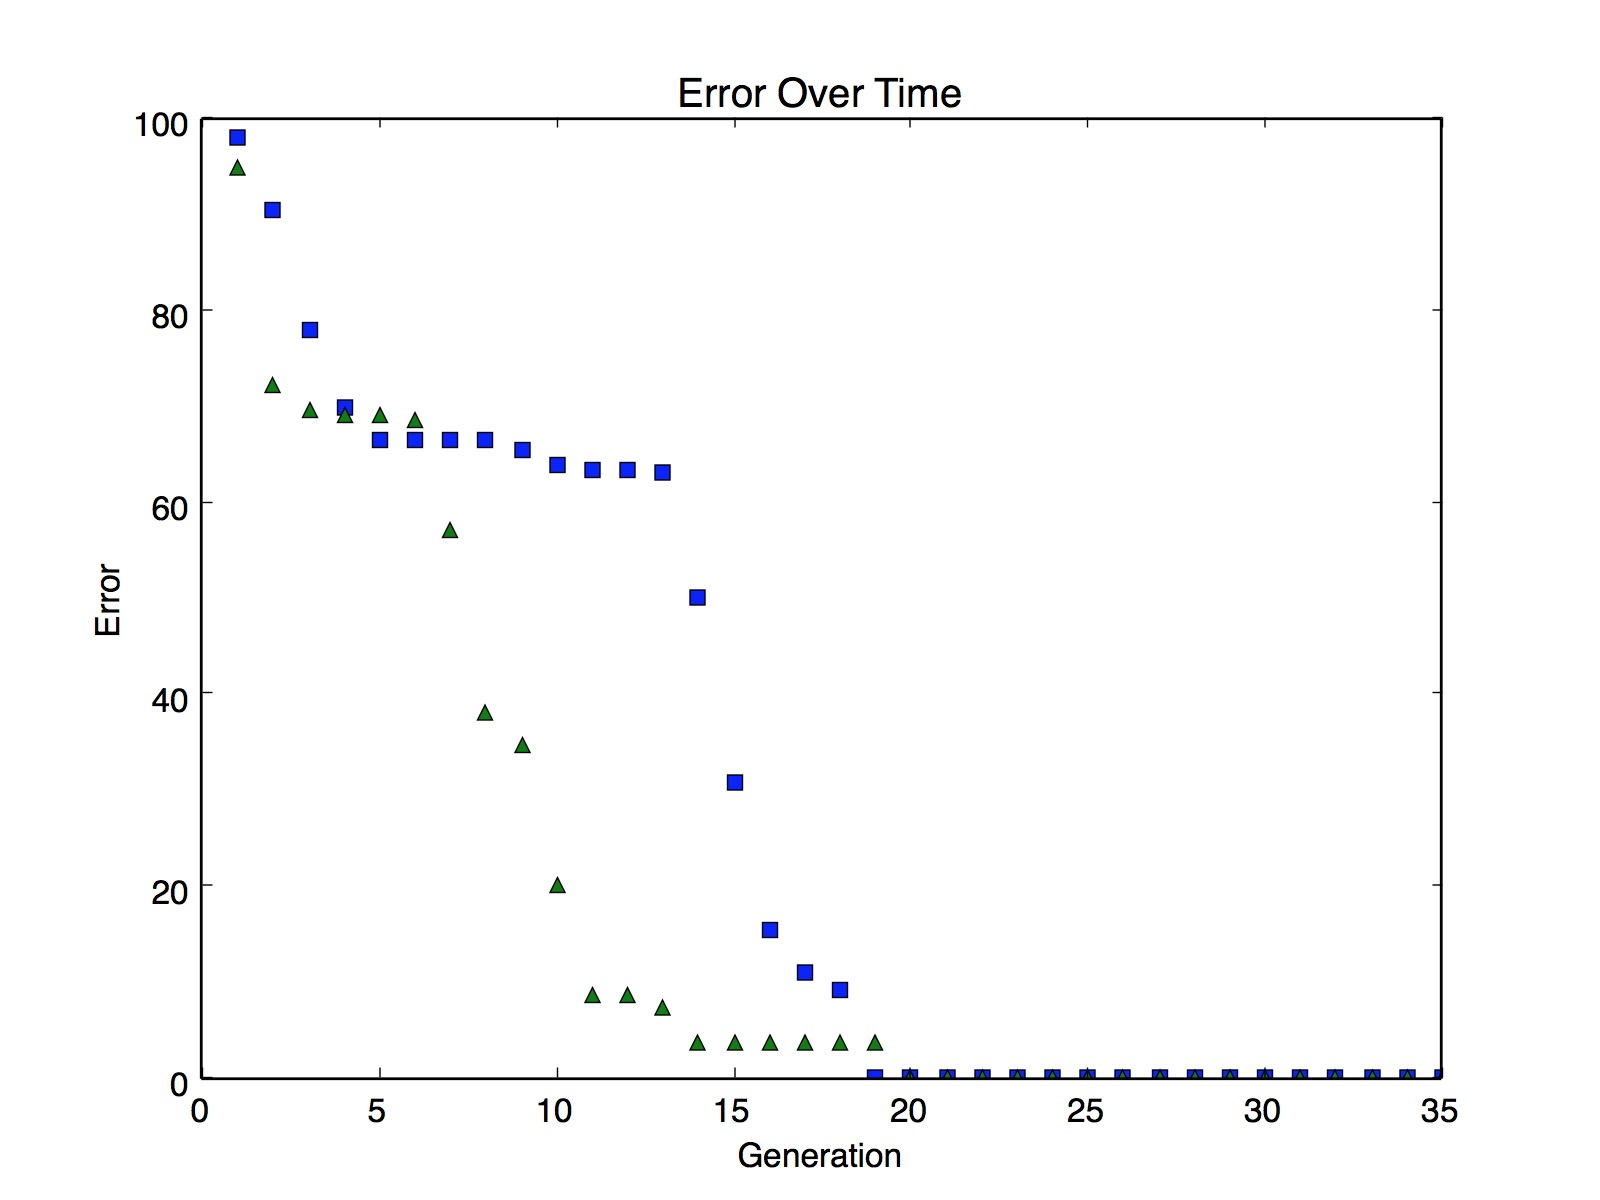
\includegraphics[width=0.5\textwidth]{figs/Generator1.jpg}

  % *Every* figure should have a descriptive caption.
  \caption{This figure depicts the best ablsolute error score for each
    generation of several genetic programming runs. Each of the runs
    depicted were the best runs of a full experimental run of 10 runs of
    genetic programming.}


  \label{fig:tex}

\end{figure}


\section{Conclusions}
\label{sec:concl}

We began with the goal of developing a program that could estimate a
function using Symbolic Regression analysis for two different
datasets. We used standard genetic programming practices to evolve
random functions into reasonable estimates of a function for each
dataset. The most notable aspects of our program are: the initial
population size of 1000, reproduction rate of 10\%, a point
mutation rate of 40\% in 10\% of each population, and random crossing
over between individuals selected by tournament selection.\\

Over all the independent runs on the dataset from Generator 1, we only
converged on a function with non-existant error for the test set and
training set once. However, our algorithm never found a function for
the three variable dataset with an absolute error less than 400
million. Given our results, we
believe our program is only capable of estimating single variable
functions with any reliable accuracy. \\

In future experiments, a larger generation size and a greater number of generations should be used to evolve a solution. Additionally, a secondary selection criterion similar to the order of nonlinearity selection proposed by Vladislavleva et al would be beneficial for more accurate estimations, especially for multivariable functions \cite{Vladislavleva:2009:ONC:1650356.1650365}.
%
\section{Acknowledgements} 
\label{sec:ack} 

This section is optional. But if there are people you'd like to thank for their help with the project --- a person who contributed some insight, friends who volunteered to help out with data collection, etc. --- then this is the place to thank them. Keep it short!


% This creates the refereces section. Open the project1.bib file to
% see how to organize your references.
\bibliography{project1}
\bibliographystyle{aaai} % sets citation and bib style, do not modify

\end{document}
